% !TEX root = ../thesis.tex

In this chapter we discuss how the Expectation Propagation (EP) algorithm can be exploited when attempting to perform (approximate) Bayesian inference with distributed data. 
We focus on how different variants of the EP algorithm perform, how amenable they are to scaling and how robust they are to noisy estimations of the EP updates. 

%%%%%%%%%%%%%%%%%%%%%%%%%%%%%%%%%%%%%%%%
\section{Distributed Bayesian Inference}

In this section we consider the problem of performing Bayesian inference when the relevant data is distributed across different compute nodes. 
Let us assume that there are $K$ such compute nodes each holding independent parts of the data $y_i$ (with $i=1,\dots,K$), such that these parts form a partition of the complete data $y$. 
In a Bayesian setting, we are interested in the posterior distribution over a parameter of interest $x$ given the entire data $y$. We can write this posterior as the product of $K$ terms corresponding to the parts $y_i$: \check{june8, aug17}
%
\eqa{
	p(x\st y) &\propto& \pi_0(x) \prod_{i=1}^{K} p(y_i\st x)\label{eq:distrposterior}
}
%
where $\pi_0$ is a prior distribution. Each of the likelihood terms itself factors over the individual data points of $y_i$, i.e.: $p(y_i\st x)=\prod_{j=1}^{N_i}p(y_{ij}\st x)$ with $N_i$ the number of individual data points held by the $i$th compute node.

It is important to stress that, in the setup considered here, each compute node only has access to independent subsets of the data. In \citet{hasenclever16} we explain that this situation can occur in large scale learning but also in cases when the data cannot be shared directly (e.g.: for privacy reasons). This type of context is sometimes known as divide-and-conquer or consensus inference \citep{kleiner14,battey15,zhao16}. 

Defining $t_i$ to be nonnegative factors with $t_i(x)=p(y_i\st x)$, the factorised form \eqref{eq:distrposterior} reads $\pi_0(x)\prod_{i=1:K}t_i(x)$ which is the form \eqref{eq:targetfactorises} that we had used to motivate the introduction of the ADF and EP algorithms (cf.\ section \ref{s:ADF+EP}).
In the rest of this chapter, we show how different variants of the EP algorithm can be used to perform parallel variational inference in the presence of distributed data.\check{jul25,jun8, aug18} 

%%%%%%%%%%%%%%%%%%%%%%%%%%%%%%%%%%%%%%%%%%%%%%%
\section{\label{sec:ep-for-dbi}EP variants for Distributed Inference}
The target distribution of interest has the form $p(x)\propto \pi_0\prod_{i=1:K}t_i(x)$ where the evaluation of one of the $t_i$ requires access to the compute node $i$. The aim is to construct an approximation $q\in\mathcal F_\phi$ parametrised by a vector $\theta$ with\footnote{we included a prior here unlike in \eqref{eq-log-partition}, the log-partition function is therefore implicitly understood to consider the prior as well with
$$
	A(\theta) \esp=\esp \log \int \pi_{0}(x)\exp\scal{\theta,\phi(x)}\nudx
.
$$}
%
\eqa{
	q_{\theta}(x) &=& \pi_0(x)\exp(\scal{\theta,\phi(x)}-A(\theta)) \spe \pi_0(x)\exp(-A(\theta))\prod_{i=1}^{K}\tilde t_i(x)
}
%
where $\tilde t_i(x):=\exp\scal{\omega_i,\phi(x)}$ for parameters $\omega_{i}$ such that $\sum_{i=1:K}\omega_i=\theta$. The tilted distributions associated with each of the factors are given by
%
\eqa{
	q_i(x) &=& \pi_0(x)t_i(x)\exp(\scal{\lambda_i,\phi(x)}-A_i(\lambda_i))
}
% 
where $\lambda_i=(\theta-\omega_i)$ and $A_i(\lambda_i)$ is the corresponding log-partition function. Much like the log-partition function of $q$, the $A_i$ are convex and $\nabla A_i(\lambda_i)=\E_{q_i}[\phi(X)]$. Indeed, each $A_i$ is simply the log-partition functions of the exponential-family $\mathcal F_\phi$ with respect to a modified base-measure including $t_i$.
In the EP setting, we seek to determine the parameters $\omega_1,\dots,\omega_K$ such that the LMMC \eqref{eq:LMMC} hold, i.e.: $\E_q[\phi(X)]=\E_{q_i}[\phi(X)]$ for each $i=1,\dots,K$.
The general parallel computational framework iterates on the following steps:
\begin{enumerate}\itsepa
	\item the master node sends a global parameter $\theta$ to each compute node,
	\item each compute node $i$ attempts to find a new $\omega_i$ such that the corresponding LMMC is (approximately) met and sends the updated $\omega_i$ to the master node,
	\item the master node integrates the new $\omega_i$ into $\theta$.
\end{enumerate} 

\noindent This is illustrated in figure \ref{fig:SNEP-arch} drawn from our paper \citep{hasenclever16}.

\begin{figure}[!h]
	\center
	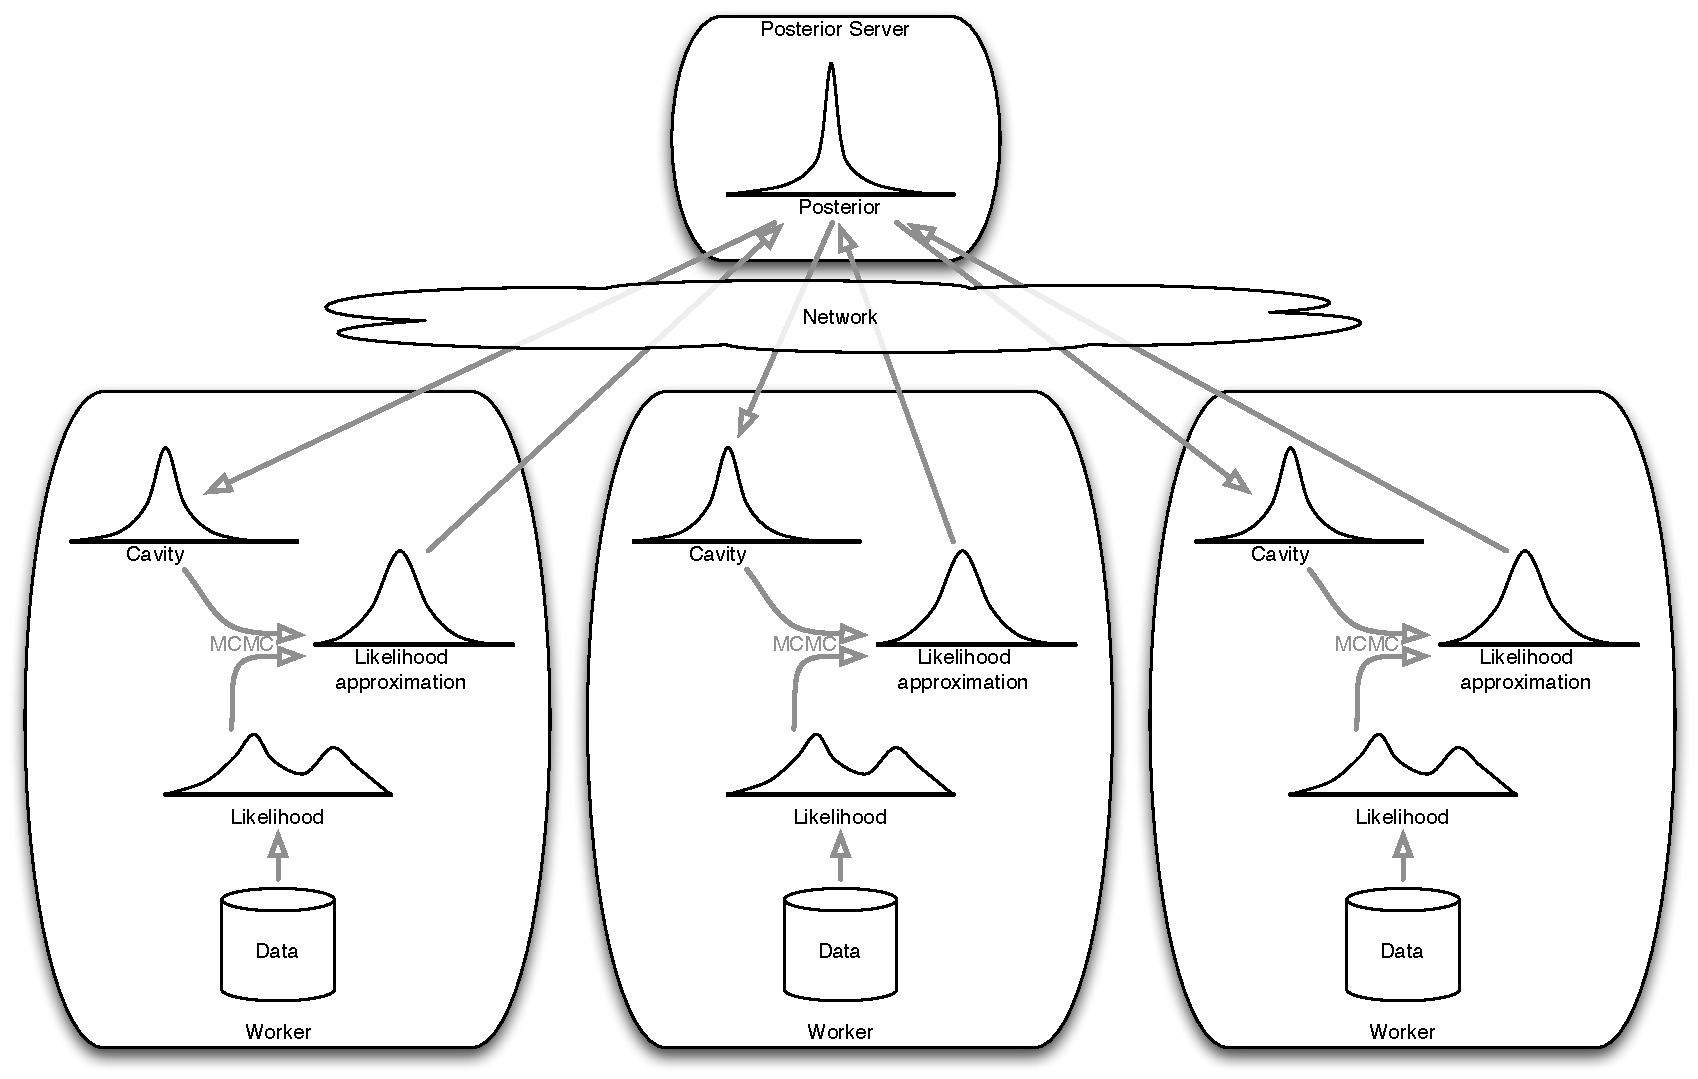
\includegraphics[width=\textwidth]{figures/snep/PosteriorServer}
	\caption{\label{fig:SNEP-arch} Illustration of the use of EP as the backbone for distributed Bayesian learning. Each compute node or worker (bottom) has access to its data and can compute the likelihood of that data. Including the cavity retrieved from the master and projecting on the exponential family leads to an approximation of the global likelihood which can be sent back to the master and combined with other such approximations sent back by the other workers.}
\end{figure}

As we will see, there are different ways to implement this general framework.
We will show empirically that a determining element in the performance of a particular implementation is its robustness to Monte Carlo noise. 
Indeed, in our general setting we do not assume that computing $\E_{q_i}[\phi(X)]$ can be done exactly. Rather, we assume that it is approximated by a Monte Carlo estimator.\check{june8, aug18}
%%%%%%%%%%%%%%%%%%%%%%%%%%%%%%%%%%%%%%%%%%%%%%%%%%%%%%%%%

\subsection{Damped updates in the natural parameter space}
In their paper, \citet{xu14} suggest a method to synchronise Monte Carlo samplers running on independent compute nodes. 
They call it \emph{Sequential Moment Sharing} or SMS for short. 
It was originally proposed to scale up MCMC methods and as such it assumes that MCMC chains can be run for many iterations to convergence in between communications with the master. Effectively, SMS corresponds precisely to the case mentioned at the previous point consisting of running EP across multiple physical nodes while using noisy estimates of $\E_{q_i}[\phi(X)]$, the expected value of the sufficient statistics under the tilted distribution. 
Below, we introduce the algorithm as a damped fixed-point iteration in the natural parameter space. This will prove useful when comparing different EP-like algorithms.\check{june8,may27, aug18}

We showed that the basic EP algorithm could be interpreted as a kind of fixed point iteration targeting the Local Moment Matching Conditions \eqref{eq:LMMC} (LMMC). At a given step of the algorithm, when considering the inclusion of the factor $t_i$, the global parameter should therefore be updated such as to verify $\E_{q_\theta}[\phi(X)]= \E_{q_i}[\phi(X)]$. Let us define the moment of the local tilted distribution as $\mu_i:=\E_{q_i}[\phi(X)]$, the update then amounts to finding $\theta$ such that $\nabla A(\theta) = \mu_i$ or
%
\eqa{	
	\theta &\leftarrow & \nabla A^{\star}(\mu_i).	\label{eq:ep-np-update}
}
%
In the case where one is considering a Monte Carlo estimator for $\mu_i$, these updates are inexact and it is crucial to mitigate the effect of the noise by considering \emph{damped updates}. In fact, even when one uses the exact $\mu_i$, it can be beneficial to the overall convergence of the algorithm to consider damped updates \citep{heskes03}. Damping \eqref{eq:ep-np-update} leads to the modified update:\check{may11}
%
\eqa{
	\theta &\leftarrow & (1-\kappa)\theta + \kappa \nabla A^{\star}(\hat\mu_i),\label{eq:damped-update-np}
}
%
where $\kappa \in(0,1]$ is the damping parameter and $\hat\mu_i$ is an estimator for $\mu_i$. As in the gradient descent algorithm, the damping parameter can be decreased over iterations according to a schedule in order to further help convergence (in point \ref{point:MD-for-EP} we expose in more details how EP can be understood in a gradient descent framework).
The damped update \eqref{eq:damped-update-np} can also be expressed in terms of the $\omega_i$ (parameter of the factor approximation $\tilde t_i$) and the $\lambda_i$ (parameter of the corresponding cavity):\check{june8}
%
\eqa{
	\omega_i &\leftarrow& \omega_i + \kappa(\nabla A^{\star}(\hat\mu_i)-\lambda_i).\label{eq:damped-update-np-w}
}
%
One can also swap the role of $\lambda_i$ and $\omega_i$ and obtain another valid damped update mechanism. Both forms are amenable to parallelisation since they can be expressed solely in terms of local parameters attached to the $i$th compute node.%\add{review statement after experiments, potentially in lambdai less stable because cavity collapse but should check if can explain why}\check{june8,may27}

The basic SMS algorithm operates synchronous updates.
At step $k$, each node receives the current global parameter $\theta$ and computes the parameter corresponding to the current tilted distribution $q_i$ i.e.: $\lambda_i=(\theta-\omega_i)$. Each node then forms a Monte Carlo estimator $\hat\mu_i$ of $\E_{q_i}[\phi(X)]$, computes the damped step \eqref{eq:damped-update-np-w} and returns the updated local parameter $\omega_i$ to the master node. 
The master node then aggregates all updated local parameters and updates the global parameter: 
%
\eqa{	\theta &\leftarrow& (1-\kappa')\theta+\kappa'\sum_{i=1}^{K}\omega_{i}	}
%
where $\kappa' \in (0,1]$ is a global damping parameter which may also help overall convergence. 
These steps are summarised at the algorithm \ref{alg:ep-sms-synch} below.\check{june8}

\begin{algorithm}[!h]\small
	\caption{\label{alg:ep-sms-synch}\dblue{\emph{\small Sequential Moment Sharing (synchronous)}}}
	\begin{algorithmic}[1]
	\State Initialise $\theta,\omega_{1},\dots,\omega_{K}$ such that $\theta=\sum_{i=1}^{K}\omega_{i} \in \Omega$ and send to each compute node
	\For{$k=1:N_{\text{EP}}$}
		\State Send current global parameter $\theta$ to each node
		\For{node $i=1:K$}
			\State Update the cavity parameter $\lambda_{i}\leftarrow\theta-\omega_{i}$
			\State Form an estimator $\hat\mu_{i}$ of $\E_{q_{i}}[\phi(X)]$
			\State Update the local parameter $\omega_{i}\leftarrow\omega_{i}+\kappa(\nabla A^{\star}(\hat\mu_{i})-\lambda_i)$
			\State Send the updated $\omega_{i}$ to the master node
		\EndFor
		\State Update global parameter $\theta\leftarrow (1-\kappa')\theta + \kappa'\sum_{i=1}^{K}\omega_{i}$
	\EndFor\\	
	\Return{$\theta$}
	\end{algorithmic}
\end{algorithm} 

It is easy to see how this algorithm can be altered to accommodate asynchronous updates. Indeed, instead of waiting for all nodes to complete their tasks, each node could asynchronously request the most recent global parameter $\theta$ available from the master node while the master node would continuously integrate information it receives from the compute nodes. In fact, each node would then simply send the difference $\delta_{i} = (\omega_{i}^{\text{new}}-\omega_{i}^{\text{old}})$ which can be integrated directly into an update of $\theta$. \check{june8}

%%%%%%%%%%%%%%%%%%%%%%%%%%%%%%%%%%%%%%%%%%%%%%%%%%%%%%%%%
\subsection{Damped updates in the mean parameter space}

The main issue with the SMS algorithm which we will expose in more details in the experiments (see section \ref{dist-ep-exps}) is that it performs the projection of the noisy estimator $\hat\mu_{i}$ \emph{before} the damping step. Since this projection operator is in general non-linear and potentially numerically unstable (in the Gaussian case, for example, it requires a matrix inversion) this can hinder the performances of the algorithm. In the case of the Gaussian distribution for instance, the projection effectively requires the inversion of a noisy matrix (see \eqref{proj-mp-np-gauss}). It seems therefore sensible to suggest damping the estimator \emph{before} it gets projected. This leads to going from \eqref{eq:damped-update-np} to\check{june11}
%
\eqa{
\nabla A(\theta) &\leftarrow& (1-\kappa)\nabla A(\theta) + \kappa \hat\mu_{i}
}
%
or, equivalently, to
%
\eqa{
\theta &\leftarrow& \nabla A^{\star}(\nabla A(\theta) + \kappa (\hat\mu_{i}-\nabla A(\theta))).
\label{eq:damped-update-mp}
}
%
Of course, if $\kappa=1$ (no damping), both approaches are equivalent. Readers familiar with convex optimisation will also notice the similarity with the \emph{mirror-descent algorithm} \citep{nemirovski83, beck03}. We will explore and discuss this similarity later in point \ref{point:MD-for-EP}. 
These updates can also be expressed in terms of updates of the local parameters:
%
\eqa{
\omega_{i} &\leftarrow& \nabla A^{\star}(\nabla A(\theta) + \kappa (\hat\mu_{i}-\nabla A(\theta))) - \lambda_{i}.
\label{eq:damped-update-mp}
}
%
As in \eqref{eq:damped-update-np-w} the role of $\omega_{i}$ and $\lambda_{i}$ can be swapped to obtain another valid damped update mechanism. 
The update \eqref{eq:damped-update-mp} can be injected into the SMS algorithm \ref{alg:ep-sms-synch} to obtain the mean-parameter variant which we will call \emph{MP-EP} to refer to the fact that the updates are done in the Mean Parameter space by contrast to \emph{NP-EP} (SMS) where the updates are done in the Natural Parameter space. 

 
%We will show below how similar updates can be obtained by considering the so-called \emph{EP-Energy} running a Newton-Raphson-like update. 

%%%%%%%%%%%%%%%%%%%%%%%%%%%%%%%%%%%%%%
\subsection{The EP energy perspective}

%%%%%%%%%%%%%%%%%%%%%%%%%%%%%%%%%%%%
%\subsubsection{Obtaining the energy}
In \citet{minka01c}, the author presents the LMMC \eqref{eq:LMMC} as a min-max problem of an objective function the author calls the \emph{EP energy function}.
One way to obtain this is to decompose the KL divergence between $p$ and $q$. 
%First, let us write explicitly the objects considered:\add{This is now REDUNDANT with start}
%\begin{itemize}\itsepa
%	\item the target distribution $p$ with $p(x)=Z_p\inv \pi_0(x)\prod_{i=1:K}t_i(x)$,
%	\item the global approximating distribution $q$ with $q(x)=Z_q\inv \pi_0(x)\exp\scal{\theta,\phi(x)}$ which we can also write $Z_q\inv \pi_0(x)\exp\scal{\sum_{i=1:K}\omega_i,\phi(x)}$ as in \eqref{eq:approxadf},
%	\item the tilted distributions $q_i$ with $q_i(x)=Z_i\inv \pi_0(x)\exp\scal{\lambda_i,\phi(x)}t_i(x)$.
%\end{itemize}
%In the list above, $\pi_0$ is the prior distribution and $Z_p,Z_q$ and $Z_i$ designate normalisation constants. From before, we have $\log Z_q=A(\theta)$ and, in a similar fashion, we can define $A_i(\lambda_i):=\log Z_i$ which enjoy similar property as $A$. In particular, it is convex and $\nabla_{\lambda_i} A_i(\lambda_i) =\mu_{i}$.\footnote{Indeed, $A_i$ is the log partition function associated with $\mathcal F_\phi$ under a modified base-measure.} The parameters of the tilted distributions $\lambda_i$ are given by $\lambda_i=(\theta-\omega_i)$ and hence must be such that $\sum_{i=1:K}\lambda_i=(K-1)\theta$.\\
To simplify notations over the next few equations we omit the dependence of the functions in $x$ which is obvious from the context; all sums and products are assumed to go over the range $i=1,\dots,K$ with $K$ the number of factors. 
The KL divergence can then be written as\check{june8,may15}
%
\eqa{	
	\KL{p,q} &=& \E_p\pac{\log\pat{Z_p\inv\pi_0\prod_{i}t_i}-\log q}	.
\label{eq:decomposeKL}}
%	
Consequently, the product $t_i$ can be manipulated to make the $q_i$ appear:
%
\eqa{
	\prod_{i} t_i &=& \prod_{i}{\pi_0\exp\scal{\lambda_i,\phi}t_i\over \pi_0\exp\scal{\lambda_i,\phi}}\spe {\prod_i Z_iq_i\over \pi_0 (Z_q q)^{K-1},}
}
%
and using this in \eqref{eq:decomposeKL} leads to:\footnote{Note that considering the reverse KL leads to a very similar decomposition:
\[\KL{q,p} - \log Z_p \spe -\mathcal E + \sum_i \KL{q,q_i}.\]}
%
\eqa{
\KL{p,q} + \log Z_p &=& {(1-K) A(\theta) + \sum_{i}A_i(\lambda_i)} + \mathbb E_p\pac{\log q_i/q}.
}
%
The first part, denoted by $\mathcal E$ defines the \emph{EP energy} with
%
\eqa{
	\mathcal E(\theta,\lambda_1,\dots,\lambda_K)&=& (1-K)A(\theta) + \sum_{i=1}^{K} A_i(\lambda_i) \label{EP-energy}
}
%
under the constraint that $\theta=(K-1)\inv \sum_{i=1}^{K}\lambda_i$. Note that its gradient in $\lambda_i$ is simply $\nabla_{\lambda_i}\mathcal E = (\mu_i-\nabla A(\theta))$. 
The stationary points of $\mathcal E$ in $\lambda_i$ therefore correspond to the LMMC \eqref{eq:LMMC} that the EP algorithm attempts to satisfy.
It is also interesting to briefly look at the remainder of the right-hand side of \eqref{eq:decomposeKL}. Discarding the terms that do not depend on $\lambda_i$, we have
%
\eqa{
	\nabla_{\lambda_i}\E_p[\log q_i/q] &=& \nabla_{\lambda_i}\E_p\pac{\scal{\lambda_i,\phi}-A_i(\lambda_i)  - \scal{(K-1)\inv\sum_i\lambda_i,\phi}+A(\theta)}\nn\\
	&=& \E_{p}[\phi]-\mu_i-{1\over K-1}\E_{p}[\phi] + {1\over K-1}\nabla A(\theta).
}
%
Therefore the gradient of the complete right hand side of \eqref{eq:decomposeKL} (i.e. the gradient of $\KL{p,q}$) in $\lambda_i$ is in fact proportional to $(\E_{p}[\phi]-\nabla A(\theta))$ leading to the same stationary points as the GMMC \eqref{eq:GMMC} as could have been expected.
%
%%%%%%%%%%%%%%%%%%%%%%%%%%%%%%%%%%%%%%%%%%
%\subsubsection*{Looking for a stationary point of the EP energy}
%\todofr{Think first about how you want to present information and in particular what you want to say. Could just present the min max problem. Say that if torture the problem you can get to a double loop that looks like SNEP. Would be good not to go along the crappy road of the dev a la Teh, just showing that we're actually doing some kind of Newton's method would already be quite nice use for this \url{http://homes.soic.indiana.edu/classes/spring2012/csci/b553-hauserk/newtons_method.pdf} and probably ``Information geometry of mirror descent'' \citep{raskutti15}}

In \citet{heskes05}, the authors show that the energy \eqref{EP-energy} is in fact equivalent to their \emph{Expectation Consistent free energy}. Further, they indicate that several stationary points can exist and that the framework does not provide a criterion to pick an optimal one. Lastly, they remind the reader that since the energy is neither convex nor concave with respect to the parameters $\lambda_i$, it does not tell whether stationary points are minimum, maximum or saddle points.\footnote{So in fact, \emph{energy} is a bit of an unfortunate misnomer here.} %\check{june21}\add{should probably emphasise that ``energy'' is a bit misnomer}
%However, since the first term is concave in $\theta$ while each of the terms in the sum is convex in $\lambda_i$, \citet{minka01c} suggests writing the EP stationary points as corresponding to the following min-max problem 
%%
%\eqa{	\min	_\theta\max_{\{\lambda_i\}} \quad(K-1)A(\theta)-\sum_{i=1}^{K}A_i(\lambda_i), \quad \text{s.t.}\quad \theta = (K-1)\inv\sum_{i=1}^{K}\lambda_i.}
%
%%%%%%%%%%%%%%%%%%%%%%%%%%%%%%%%%%%%%%%%%%%%%
\subsection{\label{point:MD-for-EP}Mirror Descent for the EP energy}
Let us define $\mathcal E_i(\lambda_i)$ as the energy \eqref{EP-energy} with all parameters other than $\lambda_i$ kept fixed. On the corresponding compute node, the aim is then to determine a stationary point $\lambda_i^{\text{new}}$ for $\mathcal E_i(\lambda_i)$. This is in fact equivalent to finding a stationary point for $\mathcal G_i(\lambda_i)$ with
\eqa{
	\mathcal G_i(\lambda_i) &:=& A(\theta_{-i} + \eta\lambda_i) - \eta A_i(\lambda_i)	
}
where $\theta_{-i}:=\eta\sum_{j\neq i}\lambda_j$ and $\eta=(K-1)\inv$. A common approach to finding stationary points of a function is to consider Newton's method which revolves around a local quadratic approximation of that function. Let us denote $\lambda_i$ the current parameter and $\lambda_i^{\text{new}}$ the new one. We can consider the following development around $\lambda_i$:
%
\eqa{
\mathcal G_i(\lambda_i^{\text{new}}) 
	&\approx&
\mathcal G_i(\lambda_i) + \eta\scal{\lambda_i^{\text{new}}-\lambda_i,\nabla A(\theta)-\nabla A_i(\lambda_i)} +\nn\\
&& \qquad{\eta^{2}\over 2}\scal{\lambda_i^{\text{new}}-\lambda_i, \nabla^{2} \mathcal G_i(\lambda_i)(\lambda_i^{\text{new}}-\lambda_i)} .\label{ep-energy-newton}
}
%
Taking the gradient in $\lambda_i^{\text{new}}$ and setting it to zero then leads to a Newton-like step. However, this requires the inversion of the Hessian of $\mathcal G_i$ which may be expensive and numerically unstable to compute. An alternative can be obtained by observing that, if $\nabla^{2}\mathcal G_i(\lambda_i)$ is positive definite,\add{an argument can probably be made that this will likely be the case since if variance of q does not encompass that of qi we're in trouble (could test this), could in fact explain problems towards ``end'' of algorithm} then the quadratic term in the approximation is simply a measure of discrepancy between $\lambda_i^{\text{new}}$ and $\lambda_i$. As in the mirror-descent algorithm \citep{nemirovski83, beck03} we could therefore try to replace it by a Bregman divergence.\footnote{The Mirror Descent algorithm and its connection with the Natural Gradient algorithm is briefly covered in the appendix \ref{app:MDA+NG}).} 
In our case, it is convenient to consider the Bregman divergence induced by the log-partition function $A$ itself;\footnote{Recall that $B_A(\lambda_i^{\text{new}},\lambda_i):=A(\lambda_i^{\text{new}})-A(\lambda_i)-\scal{\lambda_i^{\text{new}},\nabla A(\lambda_i)}$.} this leads to the alternative approximation:
%
\eqa{
	\mathcal G_i(\lambda_i^{\text{new}}) &\approx&
\mathcal G_i(\lambda_i) + \eta\scal{\lambda_i^{\text{new}}-\lambda_i,\nabla A(\theta)-\nabla A_i(\lambda_i)} +\kappa\eta^{2} B_A(\lambda_i^{\text{new}},\lambda_i) \nn,
}
%
where $\kappa>0$ is a scaling factor. Taking the gradient of that approximation in $\lambda_i^{\text{new}}$ and setting it to zero then leads to a mirror-descent-like step:
%
\eqa{
	\lambda_i^{\text{new}} &\leftarrow& \nabla A^{\star}\pac{\nabla A(\lambda_i)+\kappa'(\hat\mu_i-\nabla A(\theta))}
}
%
where $\kappa'=\eta/\kappa$ can be interpreted as a step-size and $\hat\mu_i$ is a noisy estimator of $\nabla A_i(\lambda_i)$. By analogy, we can also suggest the corresponding mechanism for an update in terms of the local parameters $\omega_i$: 
%
\eqa{
	\omega_i^{\text{new}} &\leftarrow& \nabla A^{\star}\pac{\nabla A(\omega_i)+\kappa''(\hat\mu_i-\nabla A(\theta))}\label{eq:snep-updates}
}
%
which resembles the damped updates in the mean-parameter space \eqref{eq:damped-update-mp} we had obtained earlier (we will show in the experiments section \ref{dist-ep-exps} that it also underperforms compared to the updates \eqref{eq:damped-update-mp}). 
More importantly, the updates \eqref{eq:snep-updates} form the core of the \emph{Stochastic Natural gradient Expectation Propagation} (SNEP) algorithm we suggested in \citet{hasenclever16}.
%\add{Here add small discussion where you pre-announce results from experimental section}\check{june21}
The update \eqref{eq:snep-updates} can be injected into the SMS algorithm \ref{alg:ep-sms-synch} to obtain the ``SNEP'' variant we use in the experiments.
%Note that the complete algorithm presented in \citet{hasenclever16} includes a few additional elements in order to be a fully asynchronous algorithm.
 



%%%%%%%%%%%%%%%%%%%%%%%%%%%%%%%%%%%%
%
%\subsection{\dred{Parameter tying, SEP and BBa}}
%
%\todofr{
%Check if can do this cleanly: take energy, set all cavities to same (don't discuss at length explain suggestion), suggest algorithm as presented in SEP, explain how can also be done in MP space. Then same stuff with BBa. (ideally compress in one). Then discuss comparison of all stuff.
%}
%
%\subsubsection{BBA}
%\dred{DRAFT with energy set to 1}
%\eqa{	\mathcal E_{BBA}(\theta,\lambda) &=& (1-K)A(\theta)+\sum_{i=1}^{K}A_i(\lambda)	}
%under the condition that $\theta=K\lambda/(K-1)$. The stationary point of BBa 
%\eqa{	\nabla A(\theta) &=& K\inv \sum_{i=1}^{K} \nabla A_i(\lambda).	}
%(A form of average). 
%Key point is that the $\mathcal E_{BBA}$ is bounded from below for $\alpha\le N$ (see BBA) therefore convergence or something.
\clearpage
%%%%%%%%%%%%%%%%%%%%%
\section{\label{dist-ep-exps}Experiments}
%# EP exps

In this section, we compare the three main versions of EP algorithms discussed in the chapter: NP-EP where the updates are done in the natural parameter space,\footnote{This corresponds to the SMS algorithm described earlier.} MP-EP and SNEP where updates are done in the mean parameter space. For the purpose of the experiments, all algorithms are ran in a synchronous fashion. 

\subsection{Description of the experiments}

The model considered is a simple Bayesian logistic regression model. Whilst this model is of moderate interest in itself, it has the nice property of being well behaved making the analysis of the behaviour of different inference algorithms easier. This is a similar setup than the one considered in the SMS paper \citep{xu14}, generating a dataset $\mathcal D=\{(z_c, y_c)\}_{c=1}^N$ with covariates $z_c\in\mathbb R^d$ and response $y_c\in\{0,1\}$. The conditional distribution of $y_c$ given $z_c$ and weights $x\in\mathbb R^d$  is 
\begin{eqnarray}
    p(y_c=1|z_c, x) &=& \sigma(\langle z_c, x\rangle )
\end{eqnarray}
where $\sigma$ denotes the logistic function: $\sigma(s)= (1+\exp(-s))^{-1}$. A Gaussian prior $p_0(x) = \mathcal N(x; 0_d, 10\mathbb I_d)$ is set on $x$ and the aim is to construct an approximation to the posterior $p(x|\mathcal D)$. We generate $N=5000$ data points with $d=10$ using iid draws for the covariates, $z_c\sim\mathcal N(\mu, \Sigma)$ where the $d$ components of $\mu$ are drawn iid from a Uniform $\mathcal U[0,1]$ and $\Sigma=PP^T$ where the components of $P$ are drawn from a Uniform $\mathcal U[-1,1]$. The generating weight vector $x^\star$ is drawn from the prior $p_0$. The labels $y_c$ are then sampled according to the model.

The data is sharded across five factors (corresponding to 5 compute nodes) each with one fifth of the data. To compute expected values against the tilted distribution, an importance sampling estimator is constructed with a varying number of samples (5, 10, 50) as shown in figure \ref{fig-res-snep}. The proposal used is the last global approximation shared with the compute node. Note that more involved samplers can be used (as is done in \citet{hasenclever16} which uses a stochastic gradient MCMC method) but the purpose here is primarily to explore the robustness of the algorithms to Monte Carlo noise so that a simple sampler is adequate. 

All algorithms use a fixed damping throughout the iterations and different dampings were used to exhibit the behaviour of the algorithm (see \ref{fig-res-snep}). All experiments were run 5 times and averaged over those runs to account for the inherent stochasticity of the algorithms. 

As the base exponential family, we use a full-covariance Gaussian. We compare the predictive RMSE $\sqrt{\sum_c |\hat y_c-y_c|^2/N}$ obtained with $\hat y_c = \sigma(\langle z_c, \overline x\rangle)$ where $\overline x$ is the currently estimated posterior mean of the global approximation. As a reference point, we also show the RMSE corresponding to $x^\star$.

\subsection{Results}

We show in figure \ref{fig-res-snep} the evolution of the predictive RMSE with increasing number of iterations for the three algorithms considered when varying the number of iteration per samples (corresponding to the amount of Monte Carlo noise) and the damping parameter (indicated by $d=0.01$ in the legends). Note that the computational complexity of the iteration for each of the three algorithm is very similar, the main difference residing in the ordering of operations.\footnote{In all the runs, an iteration of MP-EP is around 5\% faster than an iteration of NP-EP and around 20\% faster than an iteration of SNEP but that is negligible compared to the factor of 2 speedup obtained by the much faster convergence of the algorithm.} As a baseline, the predictive RMSE corresponding to $x^{\star}$ (the generating set of weights) is drawn as a black line on each graph.

A range of damping parameters is selected to illustrate the behaviour of the algorithm. The range is always taken with the largest damping parameter being on the verge of numerical instability for the algorithm. Indeed, when using a full-covariance Gaussian as base exponential family, going from the mean-parameter space to the natural parameter space or vice versa requires the inversion of a matrix. Doing the update in the mean parameter space helps the numerical stability of this step as does increasing the damping (reducing the step-size).

It is clear from the results that the best performing algorithm is the MP-EP algorithm which converges much faster than SNEP and is much more stable than NP-EP. It is also the algorithm that offers the most robust performance in the presence of Monte Carlo noise. Finally, this algorithm corresponds to a simpler mathematical development than SNEP by being simply a mirror-descent version of the NP-EP updates. 

%%%%%%%%%%%%%%%%%%%%%%%%%%%%%%%%%%%%%
\newpage
\begin{landscape}
\begin{figure}[ht]
\vspace{-\marginparsep}
\vspace{-\marginparwidth}
\vspace*{1.7cm}
\center
%\hspace*{-2.5cm}
	\begin{subfigure}[b]{0.45\textwidth}
		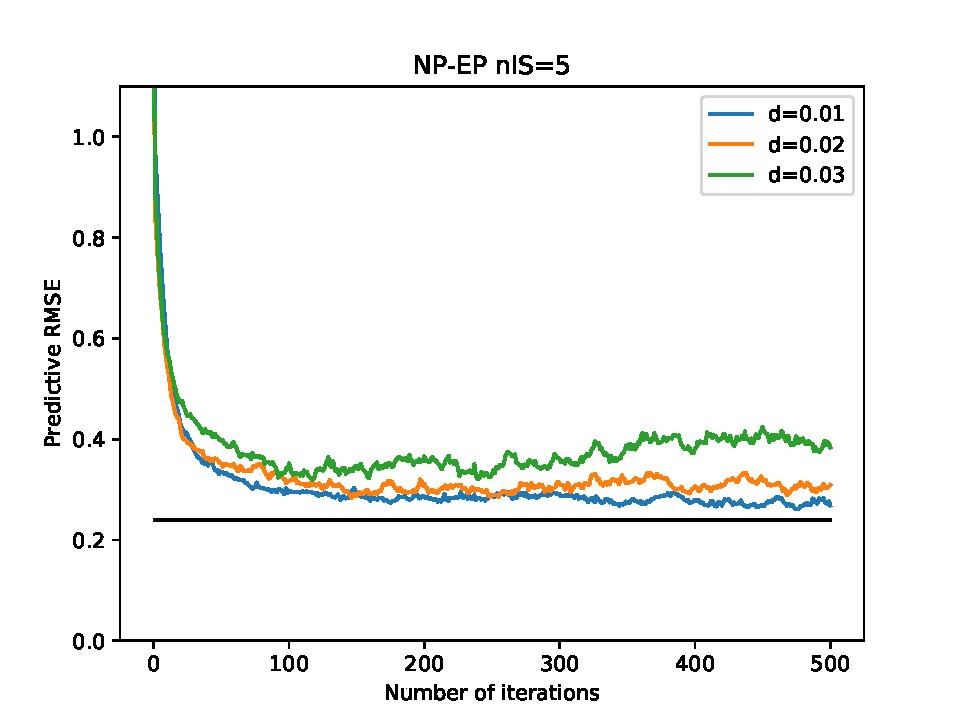
\includegraphics[width=\textwidth]{figures/snep/rms-npep-nis05}
		\caption{NP-EP, 5 samples per iter.}
		\label{res-npep-5}
	\end{subfigure}
	%\hspace*{-.5cm}
	\begin{subfigure}[b]{0.45\textwidth}
		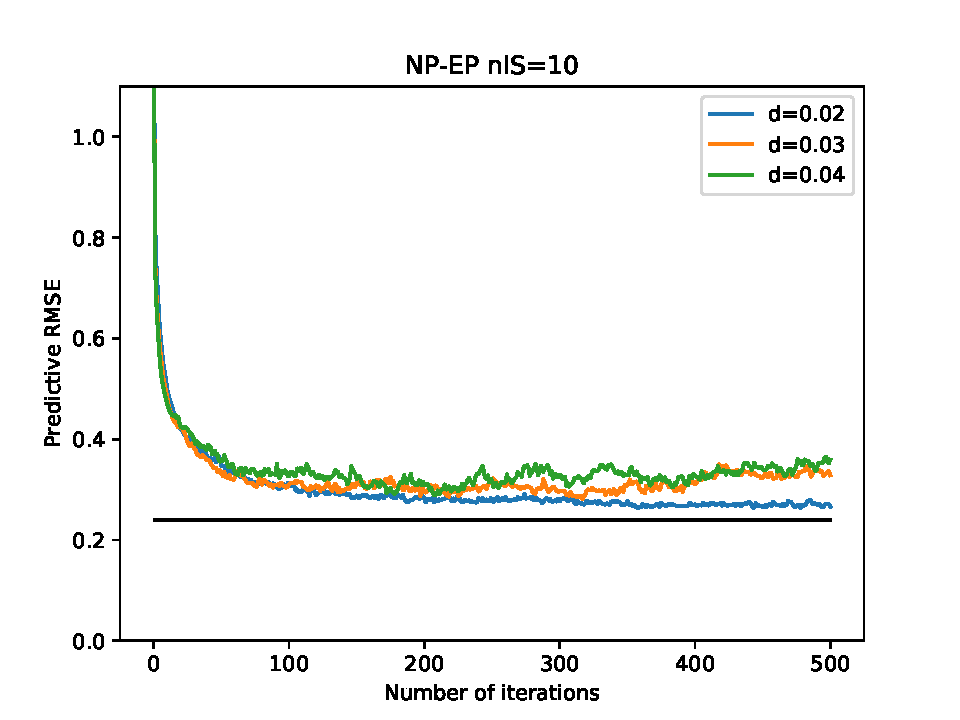
\includegraphics[width=\textwidth]{figures/snep/rms-npep-nis10}
		\caption{NP-EP, 10 samples per iter.}
		\label{res-npep-10}
	\end{subfigure}
	%\hspace*{-.5cm}
	\begin{subfigure}[b]{0.45\textwidth}
		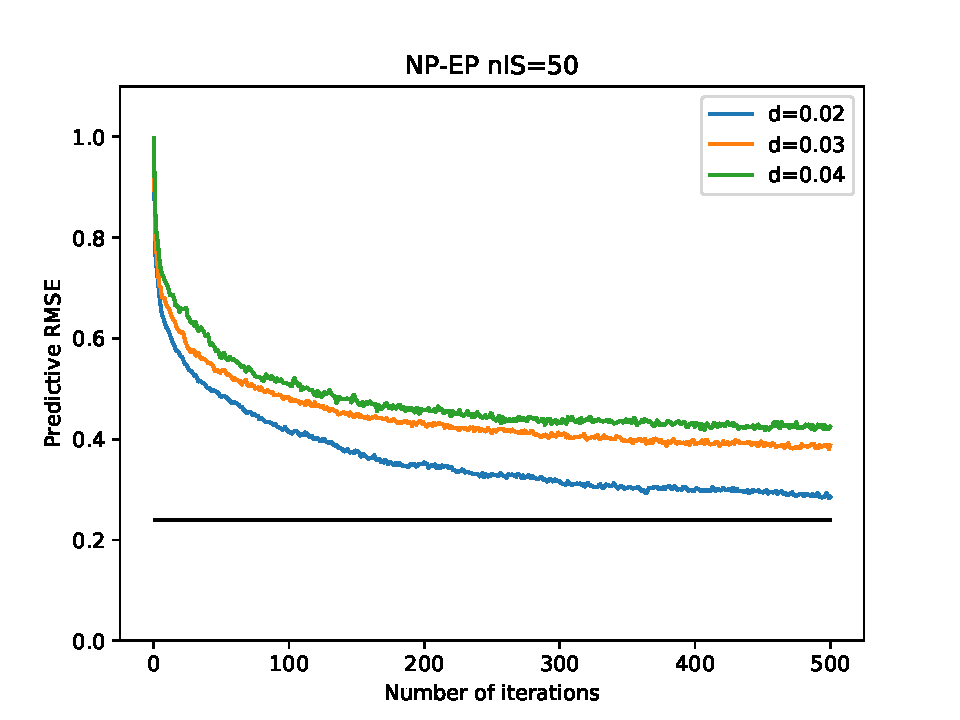
\includegraphics[width=\textwidth]{figures/snep/rms-npep-nis50}
		\caption{NP-EP, 50 samples per iter.}
		\label{res-npep-50}
	\end{subfigure}
%	
%\hspace*{-2.5cm}
	\begin{subfigure}[b]{0.45\textwidth}
		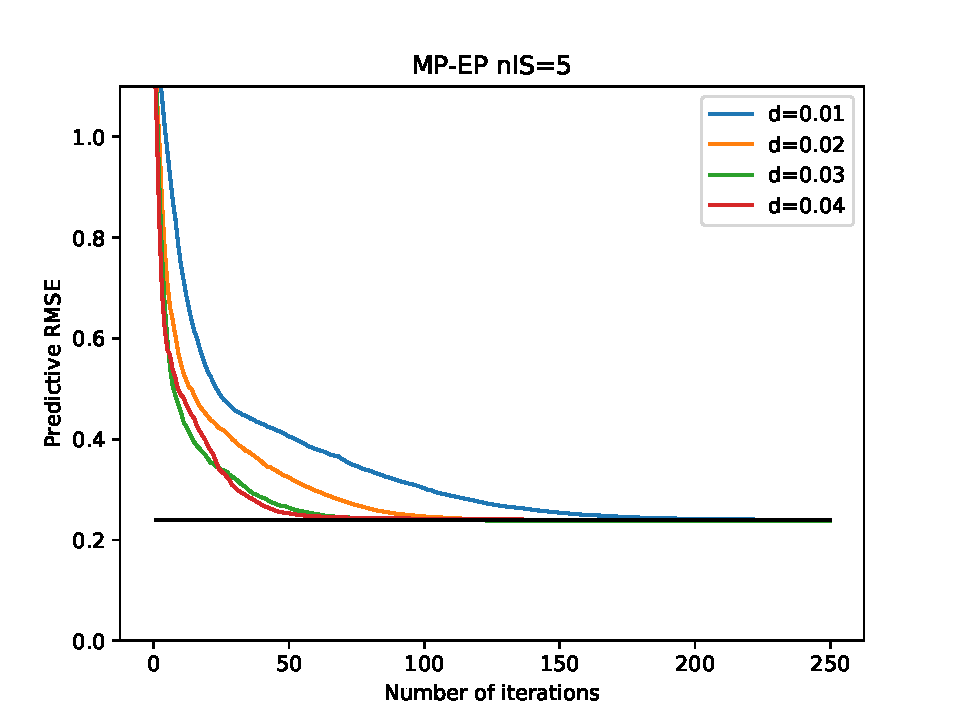
\includegraphics[width=\textwidth]{figures/snep/rms-mpep-nis05}
		\caption{MP-EP, 5 samples per iter.}
		\label{res-mpep-5}
	\end{subfigure}
%	\hspace*{-.5cm}
	\begin{subfigure}[b]{0.45\textwidth}
		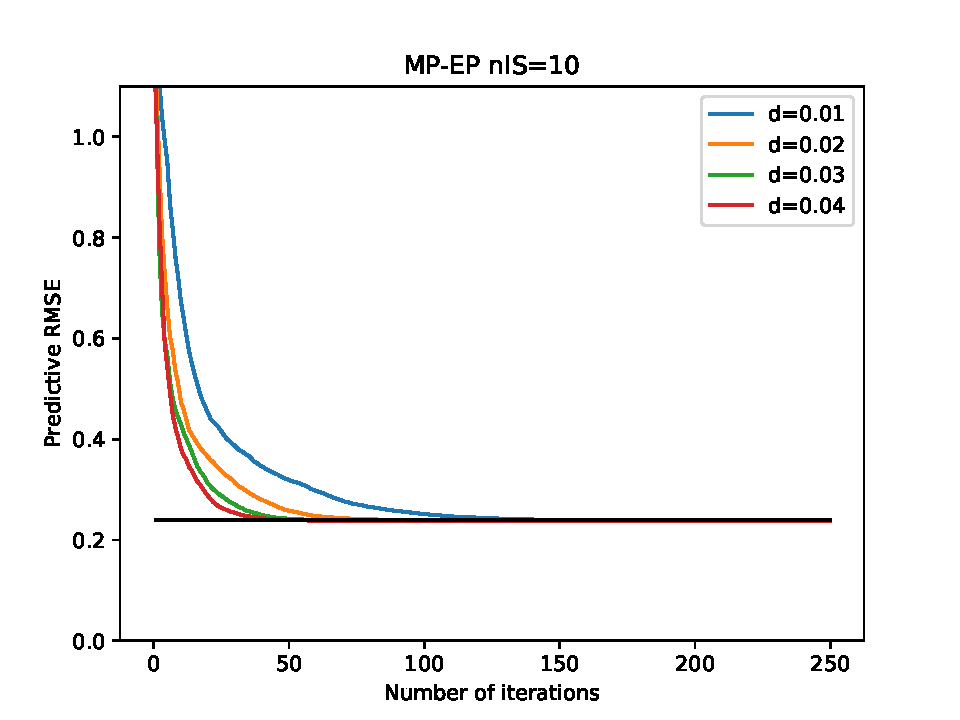
\includegraphics[width=\textwidth]{figures/snep/rms-mpep-nis10}
		\caption{MP-EP, 10 samples per iter.}
		\label{res-mpep-10}
	\end{subfigure}
%	\hspace*{-.5cm}
	\begin{subfigure}[b]{0.45\textwidth}
		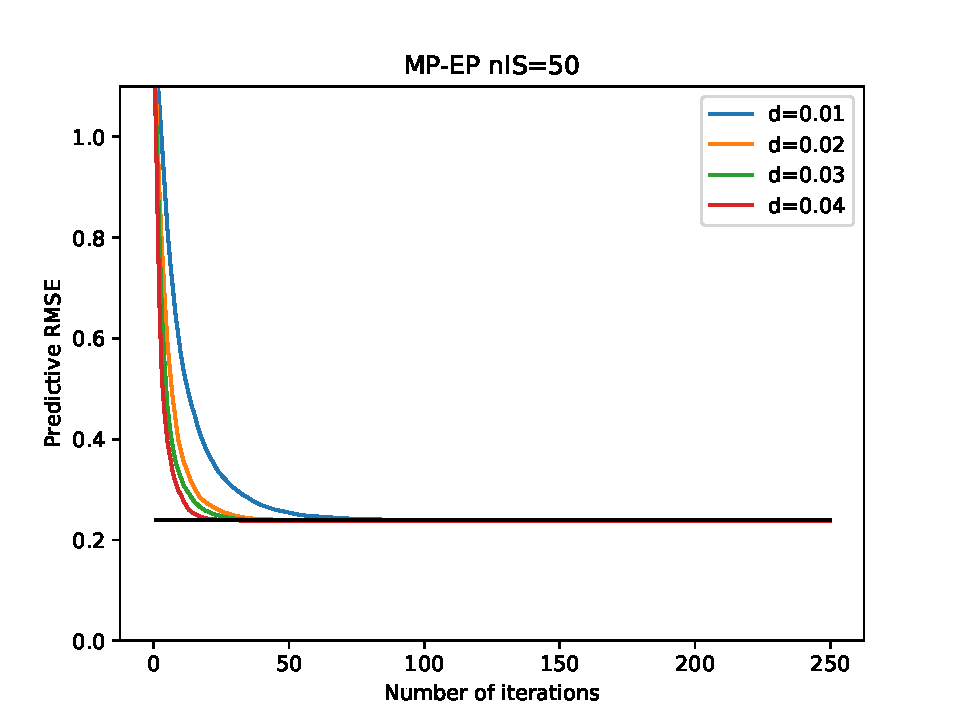
\includegraphics[width=\textwidth]{figures/snep/rms-mpep-nis50}
		\caption{MP-EP, 50 samples per iter.}
		\label{res-mpep-50}
	\end{subfigure}

%\hspace*{-2.5cm}
	\begin{subfigure}[b]{0.45\textwidth}
		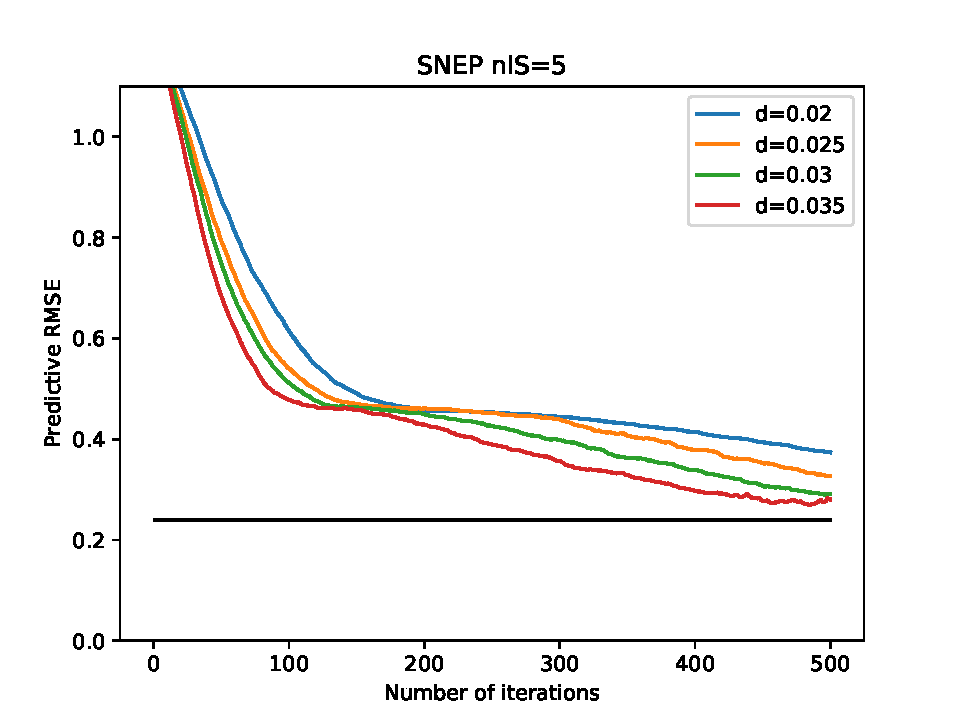
\includegraphics[width=\textwidth]{figures/snep/rms-snep-nis05}
		\caption{SNEP, 5 samples per iter.}
		\label{res-snep-5}
	\end{subfigure}
%	\hspace*{-.5cm}
	\begin{subfigure}[b]{0.45\textwidth}
		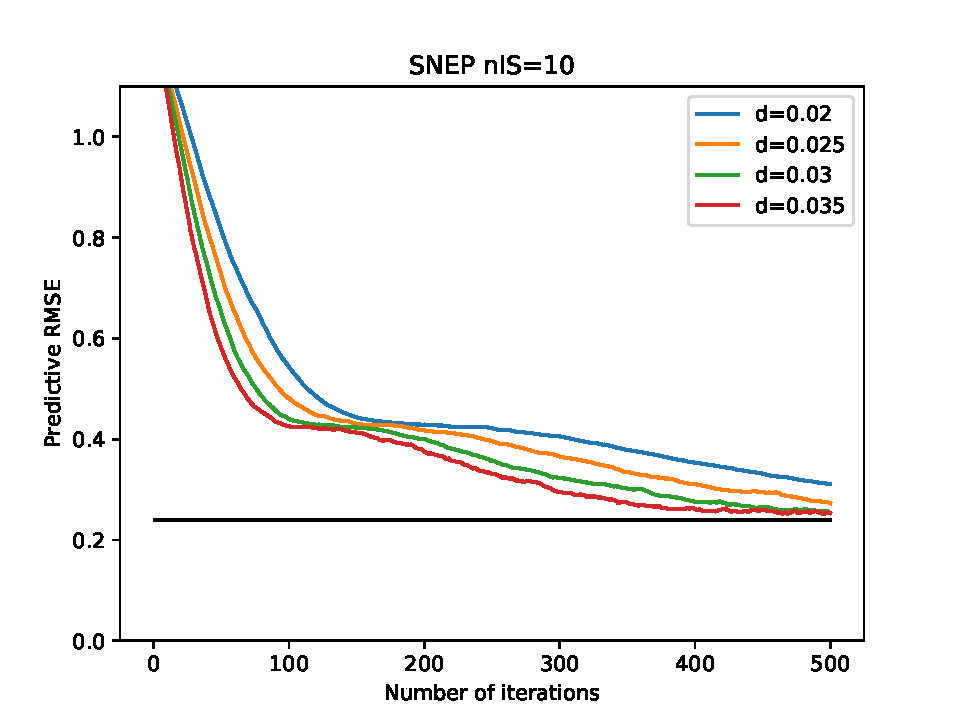
\includegraphics[width=\textwidth]{figures/snep/rms-snep-nis10}
		\caption{SNEP, 10 samples per iter.}
		\label{res-snep-10}
	\end{subfigure}
%	\hspace*{-.5cm}
	\begin{subfigure}[b]{0.45\textwidth}
		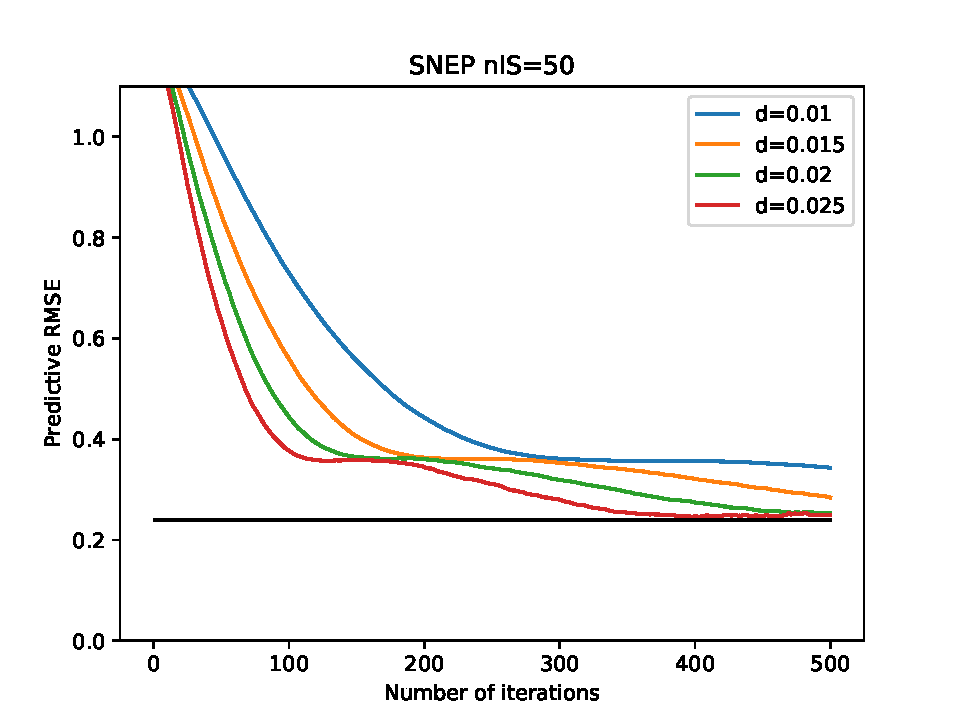
\includegraphics[width=\textwidth]{figures/snep/rms-snep-nis50}
		\caption{SNEP, 50 samples per iter.}
		\label{res-snep-50}
	\end{subfigure}		
%
\caption{\label{fig-res-snep}Results of the EP experiments (best seen in colours).}
\end{figure}
\end{landscape}
%%%%%%%%%%%%%%%%%%%%%%%%%%%%%%%%%%%%%

%\subsection{OLD}
%In this section we compare SNEP against 
%\emph{Sampling via Moment Sharing} (SMS) \citep{xu14}, a related algorithm for distributed Bayesian learning whereby each worker has a separate MCMC sampler and coordination across workers is achieved using plain EP. SMS was originally proposed to scale up MCMC methods and as such it assumes that MCMC chains can be run for many iterations to convergence in between communications with the master.  SMS uses the MCMC iterates to estimate the moments required for EP updates and so, as discussed earlier, requires a large number of iterations to produce the low Monte Carlo noise for EP updates to work properly.
%
%We illustrate below the differing dynamics of SMS and SNEP when applied to a Bayesian logistic regression model with simulated data.  We took a  similar setup as in the SMS paper \citep{xu14}, generating a dataset $\mathcal D=\{( z_{c},y_{c})\}_{c=1}^{N}$ where covariates $ z_{c}\in\mathbb R^{d}$ and response $y_{c}\in\{0,1\}$. The conditional distribution of $y_{c}$ given $ z_{c}$ and weights $ x$ is
%\begin{align}
%	p(y_{c}=1 \mid  z_{c}, x) &= \sigma( z_{c}^{\top} x)	
%\end{align}
%where $\sigma$ denotes the logistic function. 
%
%We used a Gaussian prior $p_{0}( x)=\mathcal N( x; 0_{d},10 I_{d})$ on $ x$ and the aim is to construct an approximation to the posterior $p( x \mid \mathcal D)$. We generated $N=50000$ data points  with $d=50$ using iid draws for the covariates, $z_c\sim \mathcal N(\mu,\Sigma)$ where $\mu\in[0,1]^{d}$ and $\Sigma=PP^{\top}$ with $P\in[-1,1]^{d\times d}$, with entries drawn uniformly at random for both $P$ and $\mu$. The generating weight vector $ x^*$ is drawn from the prior $\mathcal N( x; 0_{d},10 I_{d})$. The labels $y_{c}$ are then sampled according to the model. 
%
%%
%%
%Both algorithms were run with three workers, each with one third of the data. SNEP is run with 1 inner loop iteration per synchronisation with the master (for the purpose of comparing against SMS).  Varying numbers of MCMC samples per inner loop iteration were used for both algorithms, to investigate the effect of Monte Carlo noise on the performances of the algorithms (low number of samples meaning high noise and both lower performance and lower computational cost).   The damping for SMS and the learning rate for SNEP were tuned for best performances. As the base exponential family, we used a full-covariance Gaussian.  
%We compared the predictive RMSE $\sqrt{\sum_{c}|\hat{p}_{c}- y_{c}|^{2}/N}$ obtained with both methods over time where $\hat{p}_{c}=\sigma( z_{c}^{T}\overline{ x})$ where $\overline{ x}$ is the currently estimated posterior mean. We also compared the relative difference between the estimated posterior mean and that estimated from a long run of the No-U-Turn sampler \citep{hoffman14} as implemented in Stan \citep{carpenter16} with 4 chains and 50000 iterations.
%
%The \fig{fig:sms-vs-snep} illustrates the performances of both algorithms and how they are influenced by the number of MCMC samples used per iteration. It can be observed that SNEP is more robust and better performing than SMS in the presence of noise.
%In general, we found that the number of samples needed for SMS to perform well grows with the dimensionality of the problem. In models with very high dimensionality and multi-modality (e.g., neural networks), the number of samples needed per step is very large leading to iterations that are computationally impractical, whereas SNEP can afford to use many fewer samples.\\
%
%%%This can be explained by the fact that the updates in SNEP are done in the mean-parameter space and the noise is thus directly damped whereas in SMS the noisy updates are first projected in the natural-parameter space (which requires the inversion of a noisy covariance matrix) and then damped which can lead to unstable updates. 
%%%We consider the least favourable case for SNEP where only a single inner loop step is done per iteration (update \eqref{eq:meandamped}). This allows to compare fairly the number of iterations executed by SNEP and SMS since the computational cost of each iteration is similar. The results are illustrated at the figure \ref{fig:sms-vs-ep} below.
%
%\begin{figure}[!h]
%	\center
%	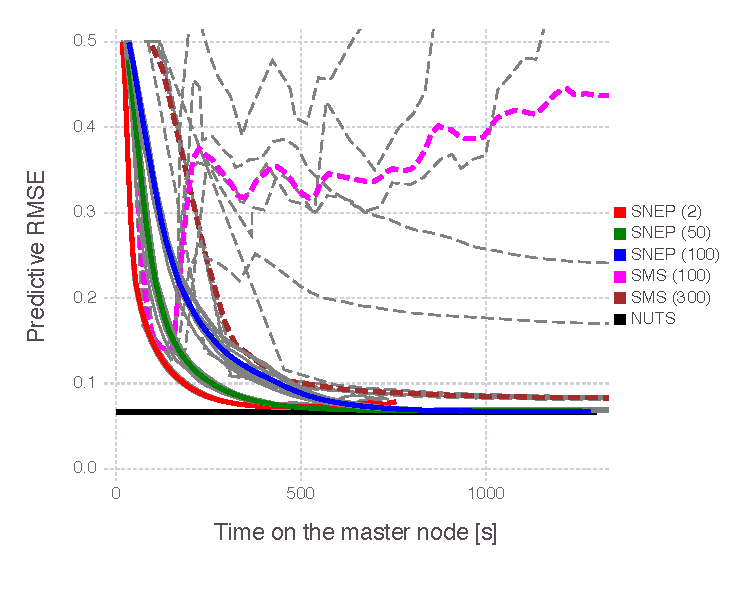
\includegraphics[width=0.65\textwidth]{figures/snep/SMSvSNEP_RMSE}
%	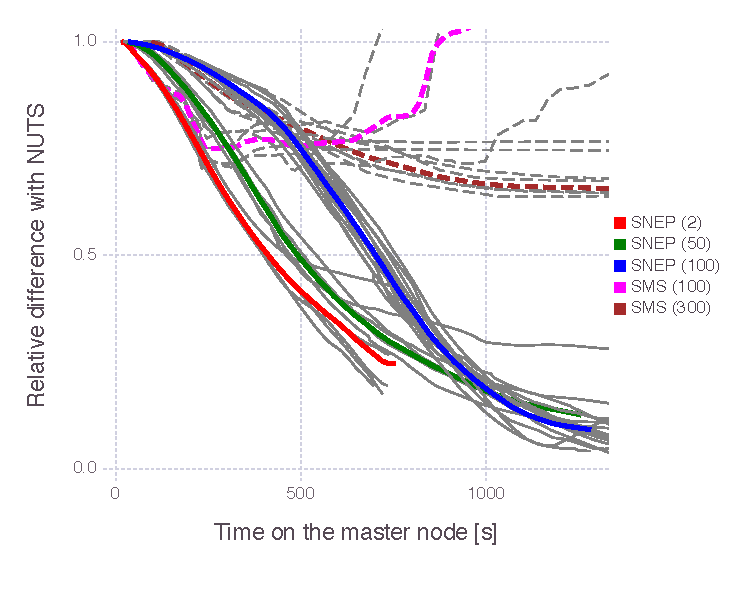
\includegraphics[width=0.65\textwidth]{figures/snep/SMSvSNEP_DIFF.pdf}
%	\caption{\label{fig:sms-vs-snep}(\textbf{top}) Comparison of the predictive RMSE obtained with SMS (dashed-lines) and SNEP (full lines) versus the time on the master node when varying the number of MCMC samples per iteration (numbers reported in the legend). When too few samples are used for the moment estimates, SMS becomes unstable whilst SNEP does not suffer from this. SNEP is also consistently faster and more accurate than SMS. The accuracy obtained with the posterior mean estimated with a long run of Stan/NUTS is also displayed as comparison (horizontal line). (\textbf{bottom}) Relative difference between the posterior means estimated using Stan/NUTS and using SMS (dashed lines) or SNEP (full lines). Each coloured line corresponds to an average over several runs (represented in light grey).}
%\end{figure}

%%%%%%%%%%%%%%%%%%%%
\section{Discussion}

In this chapter we showed that Expectation Propagation could be used as the backbone of a distributed approximate Bayesian inference mechanism. 
We showed that different variant of the EP algorithm could be used and that, in our experiments, performing updates in the mean parameter space can outperform updates in the natural parameter space. 
In particular we showed that updates in the mean parameter space can be much more robust to noise introduced by following inexact EP updates when the moments of the tilted distribution are computed via Monte Carlo estimators. This is particularly important for complex models where the tilted distributions are complex and sampling is very expensive so that cheap Monte Carlo estimators based on a few sampling points are favoured (e.g.: graphical models \citep{heess13, eslami14, jitkrittum15}, hierarchical Bayesian models \citep{gelman14} and approximate Bayesian computation \citep{barthelme11}). %\add{see references in confirmation with MC estimators in EP}

Since \cite{minka01}, there have been a substantial number of extensions and alternatives to EP proposed. Stochastic EP \citep{li15} and averaged EP \citep{dehaene15} assume that all factors can be well approximated by the \emph{same} exponential family factor via parameter tying. This saves memory storage and was shown to work well when a lot of samples are available. This is an orthogonal idea to our work, and it is possible to apply it to SNEP and MP-EP as well although in the distributed learning setting considered, each worker must keep a copy of the parameters anyway which means it would not reduce memory requirements. Convergent EP \citep{heskes03} is a similar algorithm with (idealised) convergence guarantees but it is extremely slow to run in practice. 

A critique often raised against EP is that the algorithm does not offer convergence guarantees. In fact, Minka addresses this in his paper \citep{minka01} indicating that when EP does not converge it is usually a sign of a poor choice of approximating family $\mathcal F_{\phi}$. 
Further to this, the convergence question may in fact be of little practical use since, in any case, we do not know how good an approximation the fixed point corresponding to the local moment matching conditions (LMMC) is to the fixed point corresponding to the global ones (GMMC) nor how good a proxy the latter is to the target distribution. In fact, a similar criticism can be raised for Mean Field Variational Inference: the iterations provably decrease an energy and converge but it is unclear how good a proxy it converges to. This situation is summarised in a conceptual manner in figure \ref{comp-vi-ep}.

\begin{figure}[!h]
\center
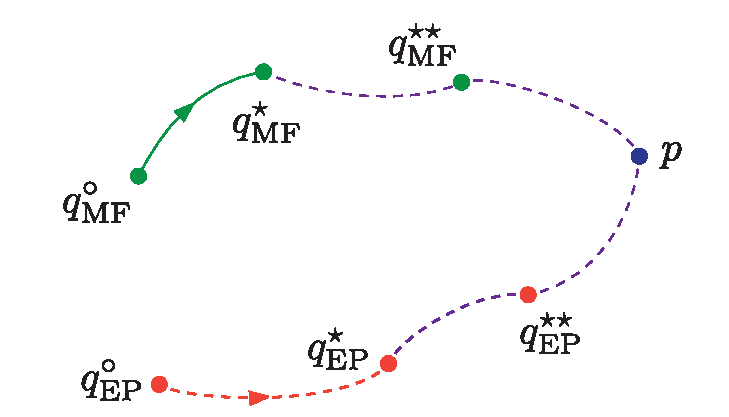
\includegraphics[width=.6\textwidth]{figures/general/vi-ep-space}
\vspace*{.2cm}
\caption{\label{comp-vi-ep}Toy representation of the approximating distributions obtained through MFVI or EP when targeting a distribution $p$ of interest. The starting points are denoted with a superscript $\circ$. MFVI provably converges to a point $q^{\star}_{\text{MF}}$ (solid green line) but we do not know how this point compares to a distribution $q^{\star\star}_{\text{MF}}$ that truly minimises the corresponding KL divergence.\\ By contrast, EP is not guaranteed to converge to a fixed point $q^{\star}_{\text{EP}}$ (dashed red line) and we also do not know how it compares to $q^{\star\star}_{\text{EP}}$ that truly minimises the corresponding KL divergence. \\
In both cases, we do not really know, in general, how the minimisers obtained compare to the target distribution $p$ (dashed purple lines). This graph is best viewed in colours. }
\end{figure}

Finally, we note that the entirety of the EP variants discussed in this section can be re-expressed in the general framework of ``Power-EP'' \citep{minka04} where the discrepancy is more general than the basic Kullback-Leibler divergence \citep{hernandez15, li16}. This, however, has little impact to the considerations discussed in the chapter in that the only element it changes is the definition of the projection operator $\mathbf P_{\phi}$. We focused on ``classical'' EP for this reason and also because, to the best of our knowledge, the role of the exponent in Power-EP is poorly understood in general.%\add{maybe add equation + discuss}



